\documentclass[journal, a4paper, onecolumn, 12pt]{IEEEtran}
\usepackage[utf8]{inputenc}
\usepackage{longtable}
\usepackage{booktabs}
\usepackage[hidelinks]{hyperref}
\usepackage{enumitem}
\usepackage{graphicx}
\usepackage{xcolor}
\usepackage{listings}
\usepackage{amsmath}
\usepackage{amssymb}
\usepackage{tikz}
\usetikzlibrary{shapes.geometric, arrows.meta, positioning, fit}

\title{Technical Report: Smart Ledger \\ \Large Integrated Database \& Financial Management Platform}
\author{\IEEEauthorblockN{Project Team}\\ \IEEEauthorblockA{\textit{Smart Ledger Project} \\ Department of Computer Science \& Engineering \\ July 2026}}

\begin{document}
\maketitle
\tableofcontents
\newpage

\section{Executive Summary}
In contemporary business operations, accurate and scalable financial ledger management is crucial. \textbf{Smart Ledger} is a cloud-native, cross-platform financial system developed to address the inefficiencies of traditional manual logging and fragmented bookkeeping. By coupling a native, high-performance frontend framework (\textbf{Flutter}) with a robust serverless backend database (\textbf{Supabase/PostgreSQL}), the system manages standard transactions while maintaining full compliance with double-entry accounting rules (GAAP/IFRS).

This technical report provides a detailed breakdown of the application architecture, database relational model, security policies, clean code structure, and functional interfaces.

\section{System Architecture}
Smart Ledger utilizes a multi-layered client-server architecture designed to support high throughput and immediate data visibility. Figure~\ref{fig:architecture} visualizes the layout of the system, highlighting the division between the user client and database back-end.

\begin{figure}[htbp]
\centering
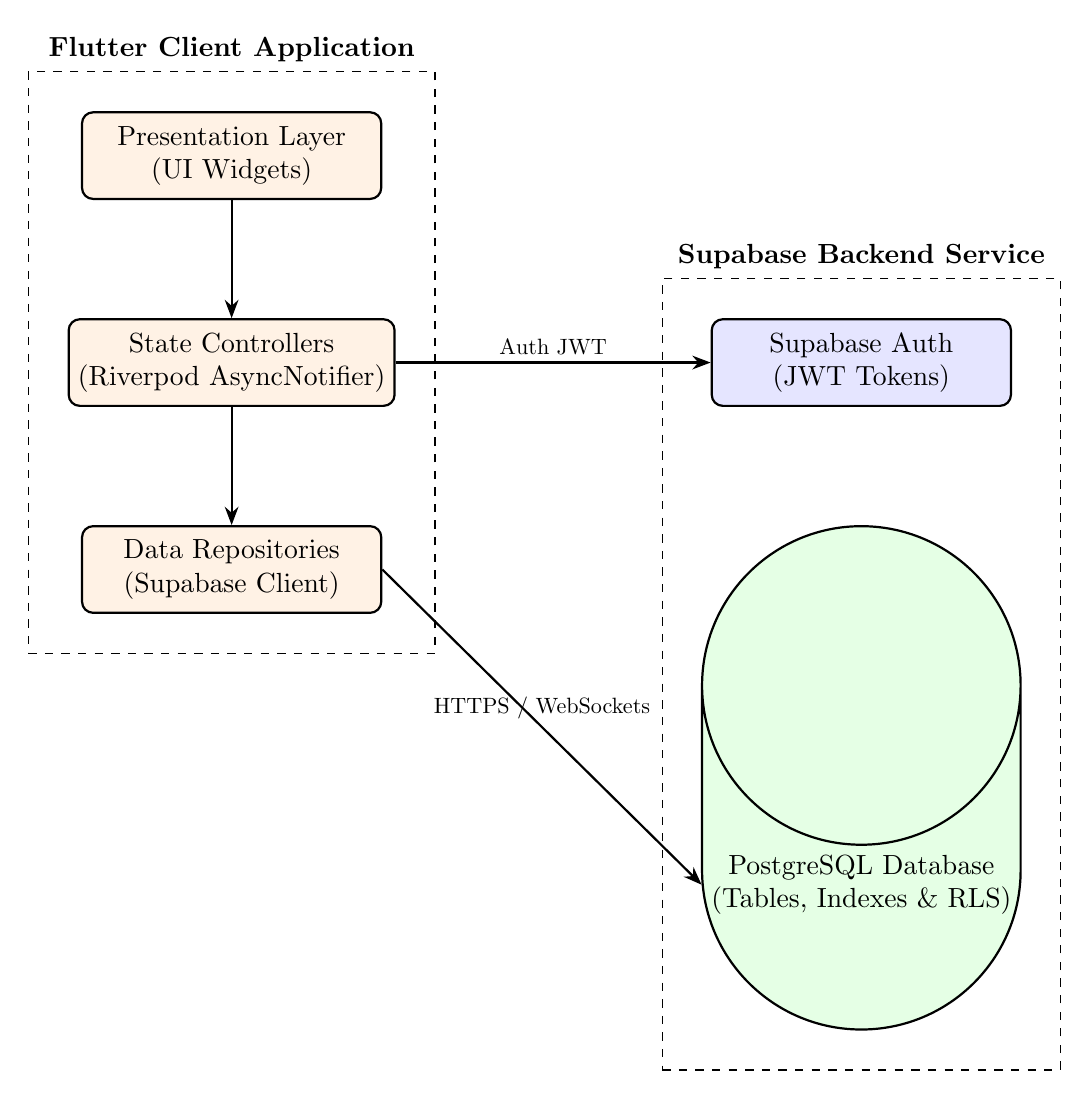
\begin{tikzpicture}[
    node distance=1.5cm and 2.5cm,
    box/.style={draw, rectangle, rounded corners=4pt, minimum width=3.8cm, minimum height=1.1cm, align=center, thick, fill=blue!5},
    dbbox/.style={draw, cylinder, shape border rotate=90, minimum width=3.2cm, minimum height=1.3cm, align=center, thick, fill=green!5},
    arrow/.style={-Stealth, thick}
]
    % Nodes
    \node[box, fill=orange!10] (ui) {Presentation Layer \\ (UI Widgets)};
    \node[box, fill=orange!10, below=of ui] (ctrl) {State Controllers \\ (Riverpod AsyncNotifier)};
    \node[box, fill=orange!10, below=of ctrl] (repo) {Data Repositories \\ (Supabase Client)};
    
    \node[box, fill=blue!10, right=of ctrl, xshift=1.5cm] (auth) {Supabase Auth \\ (JWT Tokens)};
    \node[dbbox, fill=green!10, below=of auth] (db) {PostgreSQL Database \\ (Tables, Indexes \& RLS)};
    
    % Grouping borders
    \node[draw, dashed, inner sep=0.5cm, label=above:\textbf{Flutter Client Application}, fit=(ui) (ctrl) (repo)] (client) {};
    \node[draw, dashed, inner sep=0.5cm, label=above:\textbf{Supabase Backend Service}, fit=(auth) (db)] (backend) {};
    
    % Arrows
    \draw[arrow] (ui) -- (ctrl);
    \draw[arrow] (ctrl) -- (repo);
    \draw[arrow] (repo.east) -- node[above, scale=0.8, align=center] {HTTPS / WebSockets} (db.west);
    \draw[arrow] (ctrl.east) -- node[above, scale=0.8] {Auth JWT} (auth.west);
    
\end{tikzpicture}
\caption{Smart Ledger layered client-server architecture.}
\label{fig:architecture}
\end{figure}

The layers function as follows:
\begin{itemize}[leftmargin=*]
    \item \textbf{Presentation Layer:} Implements UI elements, widgets, forms, and charts that users interact with.
    \item \textbf{State Controllers (Riverpod):} Decouples UI from data retrieval, caching data in memory, handling background transformations, and managing user interaction states.
    \item \textbf{Data Repositories:} Acts as the interface to the remote API. Handles HTTP network requests, error capturing, and parses JSON payloads to strongly typed domain objects.
    \item \textbf{Supabase Database (Postgres):} Houses the tables, manages constraint validations, indices, and ensures secure multi-tenancy.
\end{itemize}

\section{DBMS Schema \& Relational Database Analysis}
The core foundation of Smart Ledger is its relational schema. It maps simple single-entry ledger entries into structured double-entry lines to satisfy double-entry accounting constraints. Figure~\ref{fig:erd} presents the Entity-Relationship Diagram (ERD).

\begin{figure}[htbp]
\centering
\resizebox{\textwidth}{!}{
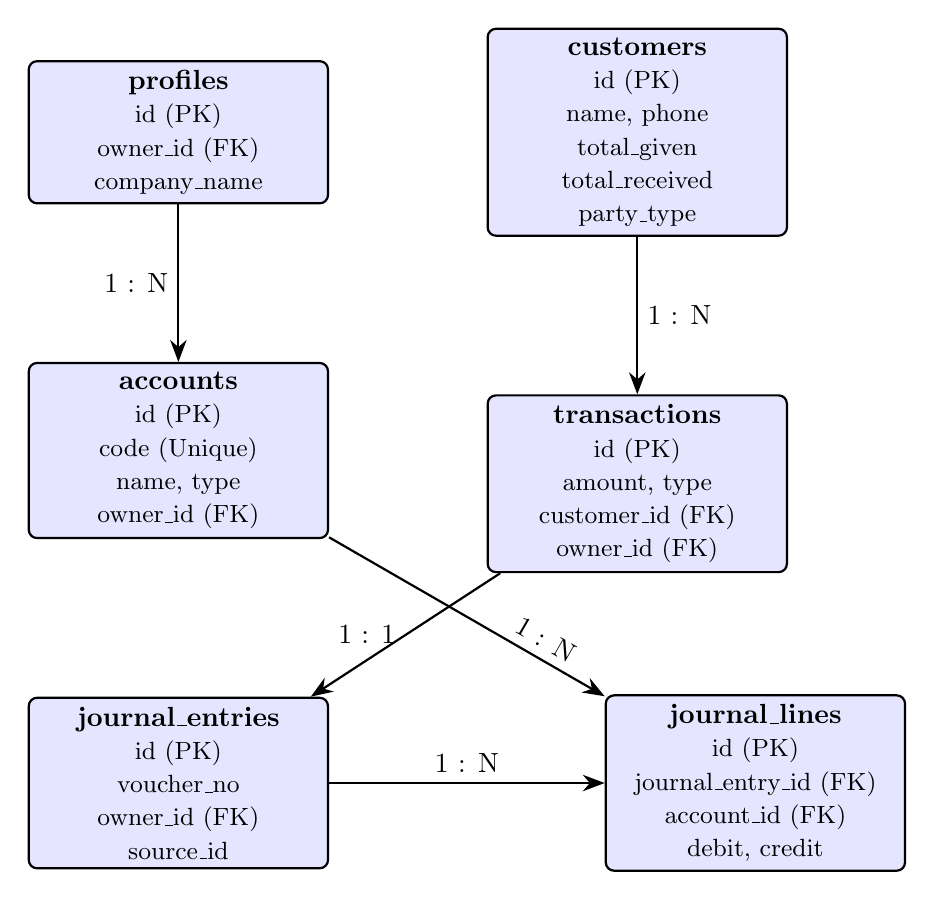
\begin{tikzpicture}[
    node distance=1.5cm and 2cm,
    entity/.style={draw, rectangle, rounded corners=3pt, minimum width=3.8cm, minimum height=1.5cm, align=center, thick, fill=blue!10},
    arrow/.style={-{Stealth[scale=1.2]}, thick}
]
    % Entities
    \node[entity] (profiles) {\textbf{profiles} \\ \small id (PK) \\ \small owner\_id (FK) \\ \small company\_name};
    \node[entity, right=of profiles] (customers) {\textbf{customers} \\ \small id (PK) \\ \small name, phone \\ \small total\_given \\ \small total\_received \\ \small party\_type};
    \node[entity, below=of customers, yshift=-0.5cm] (transactions) {\textbf{transactions} \\ \small id (PK) \\ \small amount, type \\ \small customer\_id (FK) \\ \small owner\_id (FK)};
    \node[entity, below=of profiles, yshift=-0.5cm] (accounts) {\textbf{accounts} \\ \small id (PK) \\ \small code (Unique) \\ \small name, type \\ \small owner\_id (FK)};
    \node[entity, below=of accounts, yshift=-0.5cm] (jentries) {\textbf{journal\_entries} \\ \small id (PK) \\ \small voucher\_no \\ \small owner\_id (FK) \\ \small source\_id};
    \node[entity, right=of jentries, xshift=1.5cm] (jlines) {\textbf{journal\_lines} \\ \small id (PK) \\ \small journal\_entry\_id (FK) \\ \small account\_id (FK) \\ \small debit, credit};

    % Connections
    \draw[arrow] (profiles) -- node[midway, left] {1 : N} (accounts);
    \draw[arrow] (customers) -- node[midway, right] {1 : N} (transactions);
    \draw[arrow] (accounts) -- node[midway, above, sloped, near end] {1 : N} (jlines);
    \draw[arrow] (jentries) -- node[midway, above] {1 : N} (jlines);
    \draw[arrow] (transactions) -- node[midway, left] {1 : 1} (jentries);
\end{tikzpicture}
}
\caption{Relational Database Schema Entity-Relationship Diagram (ERD).}
\label{fig:erd}
\end{figure}

\subsection{Database Tables Dictionary}
The following sections document the exact fields, data types, and primary/foreign keys used in the system:

\subsubsection{\textbf{accounts}}
Defines the structure of the chart of accounts.
\begin{itemize}[leftmargin=*]
    \item \textbf{id} (UUID, Primary Key): Unique row identifier.
    \item \textbf{owner\_id} (UUID, Foreign Key $\rightarrow$ \texttt{auth.users(id)}): Identifies the account owner.
    \item \textbf{code} (Text, Not Null): Ledger code (e.g., \texttt{1000} for Cash, \texttt{4000} for Sales Revenue).
    \item \textbf{name} (Text, Not Null): Plain text name.
    \item \textbf{type} (Text, Not Null): Constrained to: \texttt{asset, liability, equity, income, expense}.
    \item \textbf{is\_system} (Boolean, Default \texttt{false}): Restricts core ledger accounts from deletion.
    \item \textbf{created\_at} (Timestamptz, Default \texttt{now()}).
    \item \textbf{Unique Constraint:} \texttt{owner\_id, code} ensures that code values do not duplicate per user context.
\end{itemize}

\subsubsection{\textbf{journal\_entries}}
Header records containing transaction summaries and voucher details.
\begin{itemize}[leftmargin=*]
    \item \textbf{id} (UUID, Primary Key).
    \item \textbf{owner\_id} (UUID, Foreign Key $\rightarrow$ \texttt{auth.users(id)}).
    \item \textbf{voucher\_no} (Text, Not Null): Unique transaction code (e.g., \texttt{TXN-171829...} or \texttt{JV-171829...}).
    \item \textbf{date} (Timestamptz, Not Null): Timestamp of the entry.
    \item \textbf{narration} (Text): Description text.
    \item \textbf{source\_type} (Text, Default \texttt{'manual'}): Origin module (e.g., \texttt{'transaction'}).
    \item \textbf{source\_id} (UUID, Nullable): Foreign key linking back to the source transaction ID.
    \item \textbf{Unique Constraint:} \texttt{owner\_id, source\_type, source\_id} enforces a strict 1-to-1 conversion limit from cashbook records.
\end{itemize}

\subsubsection{\textbf{journal\_lines}}
Line items containing monetary distribution.
\begin{itemize}[leftmargin=*]
    \item \textbf{id} (UUID, Primary Key).
    \item \textbf{journal\_entry\_id} (UUID, Foreign Key $\rightarrow$ \texttt{journal\_entries(id)} on delete cascade).
    \item \textbf{account\_id} (UUID, Foreign Key $\rightarrow$ \texttt{accounts(id)} on delete restrict).
    \item \textbf{debit} (Numeric(14,2), Default 0.00): Cannot be negative.
    \item \textbf{credit} (Numeric(14,2), Default 0.00): Cannot be negative.
    \item \textbf{Check Constraint:} Enforces that one column contains a zero and the other contains a positive value:
    \begin{equation}
        \texttt{check ((debit > 0 and credit = 0) or (credit > 0 and debit = 0))}
    \end{equation}
\end{itemize}

\subsubsection{\textbf{customers}}
Saves client and vendor profile information and aggregate balances.
\begin{itemize}[leftmargin=*]
    \item \textbf{id} (UUID, Primary Key).
    \item \textbf{owner\_id} (UUID, Foreign Key $\rightarrow$ \texttt{auth.users(id)}).
    \item \textbf{name} (Text, Not Null).
    \item \textbf{phone}, \textbf{email}, \textbf{address} (Text, Nullable).
    \item \textbf{total\_given} (Numeric, Default 0.00): Credit given.
    \item \textbf{total\_received} (Numeric, Default 0.00): Credit paid off.
    \item \textbf{party\_type} (Text, Default \texttt{'customer'}): Constrained to \texttt{'customer'} or \texttt{'supplier'}.
\end{itemize}

\subsubsection{\textbf{transactions}}
Basic logging elements feeding cashbooks and ledger controllers.
\begin{itemize}[leftmargin=*]
    \item \textbf{id} (UUID, Primary Key).
    \item \textbf{owner\_id} (UUID, Foreign Key $\rightarrow$ \texttt{auth.users(id)}).
    \item \textbf{amount} (Numeric, Not Null): Numerical transaction value.
    \item \textbf{type} (Text, Not Null): Constrained to \texttt{'income'} or \texttt{'expense'}.
    \item \textbf{customer\_id} (UUID, Nullable, Foreign Key $\rightarrow$ \texttt{customers(id)}).
    \item \textbf{note} (Text, Nullable).
    \item \textbf{date} (Timestamptz, Not Null).
\end{itemize}

\section{Database Security \& Access Control (RLS)}
To guarantee secure isolation of client portfolios, PostgreSQL Row-Level Security (RLS) is applied to all production tables. Every select, insert, update, or delete query must validate against the active \texttt{auth.uid()} token issued by Supabase Auth.

Example SQL specifications of RLS implementations inside database migrations include:

\begin{lstlisting}[language=SQL, caption=SQL Migration excerpt for Accounts RLS policies]
-- Enable Row Level Security
ALTER TABLE public.accounts ENABLE ROW LEVEL SECURITY;

-- Select Policy
CREATE POLICY "Users can read own accounts" 
  ON public.accounts FOR SELECT
  USING (auth.uid() = owner_id);

-- Insert Policy
CREATE POLICY "Users can insert own accounts" 
  ON public.accounts FOR INSERT
  WITH CHECK (auth.uid() = owner_id);

-- Update Policy
CREATE POLICY "Users can update own non-system accounts" 
  ON public.accounts FOR UPDATE
  USING (auth.uid() = owner_id AND is_system = false)
  WITH CHECK (auth.uid() = owner_id);
\end{lstlisting}

\begin{lstlisting}[language=SQL, caption=Nested relation checks in Journal Lines policies]
ALTER TABLE public.journal_lines ENABLE ROW LEVEL SECURITY;

CREATE POLICY "Users can read own journal lines"
  ON public.journal_lines FOR SELECT
  USING (
    EXISTS (
      SELECT 1 FROM public.journal_entries je
      WHERE je.id = journal_entry_id AND je.owner_id = auth.uid()
    )
  );
\end{lstlisting}

\section{Business Logic Integration}
The transition between simple single-entry ledger tracking (used by shopkeepers or field agents) and strict double-entry balance sheets (used by accountants) is handled by the \texttt{AccountingService} module. 

When a user adds a transaction (income or expense), the system saves the raw transaction and invokes the service to record it in the ledger.

\begin{itemize}[leftmargin=*]
    \item \textbf{Credit Sale (Customer owes business):}
    \begin{align}
        \text{Debit } & \text{Accounts Receivable (Asset increase)} \\
        \text{Credit } & \text{Sales Revenue (Income increase)}
    \end{align}
    \item \textbf{Customer Payment (Got cash from client):}
    \begin{align}
        \text{Debit } & \text{Cash (Asset increase)} \\
        \text{Credit } & \text{Accounts Receivable (Asset decrease)}
    \end{align}
    \item \textbf{Direct Income (Cash sale):}
    \begin{align}
        \text{Debit } & \text{Cash (Asset increase)} \\
        \text{Credit } & \text{Sales Revenue (Income increase)}
    \end{align}
    \item \textbf{Direct Expense (Cash cost paid):}
    \begin{align}
        \text{Debit } & \text{Misc Expense (Expense increase)} \\
        \text{Credit } & \text{Cash (Asset decrease)}
    \end{align}
\end{itemize}

Double-entry integrity is enforced inside the \texttt{createJournalEntry} transaction block:
\begin{lstlisting}[language=default, caption=Dart verification for balanced journal entry]
final totalDebit = lines.fold<double>(0, (sum, line) => sum + line.debit);
final totalCredit = lines.fold<double>(0, (sum, line) => sum + line.credit);

if (lines.length < 2) {
  throw Exception('Journal entry must have at least two lines');
}
if (totalDebit <= 0 || totalCredit <= 0) {
  throw Exception('Journal entry must include debit and credit amounts');
}
if ((totalDebit - totalCredit).abs() > 0.01) {
  throw Exception('Journal entry is not balanced');
}
\end{lstlisting}

\section{Conclusion}
By establishing a robust PostgreSQL relational database with Row-Level Security, and linking frontend inputs directly to double-entry accounting journals via \texttt{AccountingService}, Smart Ledger provides a reliable, secure financial workspace. The system successfully balances ease-of-use with enterprise-grade bookkeeping standards, making it highly suitable as a DBMS project implementation.

\end{document}
